\documentclass[landscape,paperwidth=1189mm,paperheight=841mm,fontscale=0.4,margin=.7cm]{baposter}
%\documentclass[landscape,paperwidth=1682mm,paperheight=1189mm,fontscale=0.4,margin=3cm]{baposter}

\usepackage{calc}
\usepackage{graphicx}
\usepackage{amsmath}
\usepackage{amssymb}
\usepackage{relsize}
\usepackage{multirow}
\usepackage{rotating}
\usepackage{bm}
\usepackage{enumitem}
\usepackage{booktabs}
\usepackage{relsize}		% For \smaller
\usepackage{url}			% For \url

\usepackage{graphicx}
\usepackage{multicol}

%\usepackage{times}
%\usepackage{helvet}
%\usepackage{bookman}
\usepackage{palatino}
%% Pablo's personal packages
%% AMS unofficial LateX proceeding template:
%%    http://www.cimms.ou.edu/~lakshman/ametsoc/
%%\usepackage[hypertex]{hyperref}
%% end personal packages

\newcommand{\captionfont}{\footnotesize}

\graphicspath{{images/}{~/GFI/Conferences/AGU2019/AGU2019_poster/}}
\usetikzlibrary{calc}


\newcommand{\Matrix}[1]{\begin{bmatrix} #1 \end{bmatrix}}
\newcommand{\Vector}[1]{\begin{pmatrix} #1 \end{pmatrix}}

\newcommand*{\norm}[1]{\mathopen\| #1 \mathclose\|}% use instead of $\|x\|$
\newcommand*{\abs}[1]{\mathopen| #1 \mathclose|}% use instead of $\|x\|$
\newcommand*{\normLR}[1]{\left\| #1 \right\|}% use instead of $\|x\|$

\newcommand*{\SET}[1]  {\ensuremath{\mathcal{#1}}}
\newcommand*{\FUN}[1]  {\ensuremath{\mathcal{#1}}}
\newcommand*{\MAT}[1]  {\ensuremath{\boldsymbol{#1}}}
\newcommand*{\VEC}[1]  {\ensuremath{\boldsymbol{#1}}}
\newcommand*{\CONST}[1]{\ensuremath{\mathit{#1}}}

\DeclareMathOperator*{\argmax}{arg\,max}
\DeclareMathOperator*{\diag}{diag}
\DeclareMathOperator*{\argmin}{arg\,min}
\DeclareMathOperator*{\vectorize}{vec}
\DeclareMathOperator*{\reshape}{reshape}

%\font\dsfnt=dsrom12

\newcommand{\SNN}{\ensuremath{\mathbb N}}
\newcommand{\SRR}{\ensuremath{\mathbb R}}
\newcommand{\SZZ}{\ensuremath{\mathbb Z}}
%-----------------------------------------------------------------------------
% Matrices of the shape model
\renewcommand{\a}{\VEC\alpha}
\renewcommand{\v}{\VEC v}
\renewcommand{\l}{\VEC l}
\newcommand*{\m}{\VEC{\mu}}
\newcommand*{\M}{\MAT{M}}
\renewcommand*{\P}{\MAT{\Pi}}

%\newcommand{\J}{\SET J}
\newcommand{\J}{\SET{P}}
\newcommand{\Active}{\mathcal{A}}
\newcommand{\Selection}{\mathbf{S}}
\newcommand{\AllSelections}{\mathfrak{S}}
\newcommand{\Params}{\VEC\Theta}

%%%%%%%%%%%%%%%%%%%%%%%%%%%%%%%%%%%%%%%%%%%%%%%%%%%%%%%%%%%%%%%%%%%%%%%%%%%%%%%%
%%%% Some math symbols used in the text
%%%%%%%%%%%%%%%%%%%%%%%%%%%%%%%%%%%%%%%%%%%%%%%%%%%%%%%%%%%%%%%%%%%%%%%%%%%%%%%%

%%%%%%%%%%%%%%%%%%%%%%%%%%%%%%%%%%%%%%%%%%%%%%%%%%%%%%%%%%%%%%%%%%%%%%%%%%%%%%%%
% Multicol Settings
%%%%%%%%%%%%%%%%%%%%%%%%%%%%%%%%%%%%%%%%%%%%%%%%%%%%%%%%%%%%%%%%%%%%%%%%%%%%%%%%
\setlength{\columnsep}{1.5em}
\setlength{\columnseprule}{0mm}

%%%%%%%%%%%%%%%%%%%%%%%%%%%%%%%%%%%%%%%%%%%%%%%%%%%%%%%%%%%%%%%%%%%%%%%%%%%%%%%%
% Save space in lists. Use this after the opening of the list
%%%%%%%%%%%%%%%%%%%%%%%%%%%%%%%%%%%%%%%%%%%%%%%%%%%%%%%%%%%%%%%%%%%%%%%%%%%%%%%%
\newcommand{\compresslist}{%
\setlength{\itemsep}{1pt}%
\setlength{\parskip}{0pt}%
\setlength{\parsep}{0pt}%
}

%%%%%%%%%%%%%%%%%%%%%%%%%%%%%%%%%%%%%%%%%%%%%%%%%%%%%%%%%%%%%%%%%%%%%%%%%%%%%%
%%% Begin of Document
%%%%%%%%%%%%%%%%%%%%%%%%%%%%%%%%%%%%%%%%%%%%%%%%%%%%%%%%%%%%%%%%%%%%%%%%%%%%%%

\begin{document}

%%%%%%%%%%%%%%%%%%%%%%%%%%%%%%%%%%%%%%%%%%%%%%%%%%%%%%%%%%%%%%%%%%%%%%%%%%%%%%
%%% Here starts the poster
%%%---------------------------------------------------------------------------
%%% Format it to your taste with the options
%%%%%%%%%%%%%%%%%%%%%%%%%%%%%%%%%%%%%%%%%%%%%%%%%%%%%%%%%%%%%%%%%%%%%%%%%%%%%%
% Define some colors

\definecolor{silver}{cmyk}{0,0,0,0.3}
\definecolor{yellow}{cmyk}{0,0,0.9,0.0}
\definecolor{reddishyellow}{cmyk}{0,0.22,1.0,0.0}
\definecolor{black}{cmyk}{0,0,0.0,1.0}
\definecolor{white}{rgb}{1,1,1}
\definecolor{red}{rgb}{.9,0,0}
\definecolor{green}{rgb}{0,.3,0}
\definecolor{blue}{rgb}{.21,.24,.36}

\definecolor{darkYellow}{cmyk}{0,0,1.0,0.5}
\definecolor{darkSilver}{cmyk}{0,0,0,0.1}

\definecolor{middlegray}{rgb}{.4,.4,.4}
\definecolor{lightgray}{rgb}{.7,.7,.7}

\definecolor{lightgreen}{rgb}{.7,7,.35}
\definecolor{lightlila}{rgb}{.6,.6,.8}
\definecolor{lightorange}{rgb}{.88,.74,.15}
\definecolor{lighterorange}{rgb}{.98,.84,.45}
\definecolor{middleblue}{rgb}{.447,.537,.9513}
\definecolor{lightblue}{rgb}{.447,.537,.6313}
\definecolor{lighterblue}{rgb}{.568,.639,.709}
\definecolor{lighteryellow}{cmyk}{0,0,0.1,0.0}
\definecolor{lightestblue}{rgb}{.6,.7,.8}

%%% Setting Background Image %%%%%%%%%%%%%%%%%%%%%%%%%%%%%%%%%%%%%%%%%%%%%%%%%%
\background{
	\begin{tikzpicture}[remember picture,overlay]%
	\draw (current page.north west)+(-0em,0em) node[anchor=north west]
	{\includegraphics[height=1.01\textheight]{Poster_Landscape_A0_red_bg.jpg}};%{BG_ADMIRARI.jpg}};%
	\end{tikzpicture}
}


\hyphenation{resolution occlusions}
%%
\begin{poster}%
  % Poster Options
  {
  % Show grid to help with alignment
  grid=false, %true,
  % Number of columns
  columns=4,
  % Column spacing
  colspacing=1.0em,
  % Color style
  bgColorOne= red, %white, %lightgreen, %silver,
  bgColorTwo= white, %middlegray, %lightestblue, %white,
  borderColor=reddishyellow, %lightorange,
  headerColorOne= lighterblue, %lightblue, %darkSilver,  %lightblue,
  headerColorTwo=lightgray, 
  headerFontColor=black, %lightorange, %black,
  boxColorOne=darkSilver, %darkSilver, %darkblue, %darkYellow,
  boxColorTwo=white,
  % Format of textbox
  textborder=none, %faded,
  % Format of text header
  eyecatcher=true,
  headerborder=none, %open, %none,
  headerheight=0.2\textheight,
  %textfont=\sc, %An example of changing the text font
  headershape=rounded, %smallrounded,
  headershade=shadeLR,
  headerfont=\LARGE\bf,  %%\Large\bf\textsc, %Sans Serif
  textfont={\color{black}\setlength{\parindent}{1.5em}},
  boxshade=shadeTB, %shadeLR,
  background=user, %shadeTB,
  linewidth=2.5pt
  }
  % Eye Catcher
  {\begin{tabular}{c}
      \includegraphics[height=8.5em]{AGU100_logo_V-CMYK.png}\\
      \vspace{3em}
      \includegraphics[height=3.0em]{PosterNumber.png}
      
      %\includegraphics[height=4.0em]{urad2016.png}
    \end{tabular}   
  }
  % Title
  {\color{white} Uncertainties characterization of troposphere profile retrievals\\ by Bayesian inversion as compared to state-of-the-art\\ ground-based microwave radiometry methods\vspace{0.5em}}
  % Authors
  {\underline{Pablo Saavedra Garfias}$^1$ ({\color{blue} \url{pablo.saa@uib.no}})
    and Joachin Reuder$^{1,2}$\\
    $^1$Geophysical Institute, University of Bergen. Allegat{\'e}n 70, 5020 Bergen, Norway\\
	$^2$ Bjerknes Centre for Climate Research. Jahnebakken 5, 5007 Bergen, Norway\\
    %% {\color{blue} \url{www2.meteo.uni-bonn.de/admirari}}
    }
  % University logo
  {% The makebox allows the title to flow into the logo, this is a hack
   % because of the L shaped logo.
    \begin{tabular}{r}
   		\vspace{+10em}\\
      \includegraphics[height=4.5em]{UiBlogo_gray_h.png}
    \end{tabular}   
  }

%%%%%%%%%%%%%%%%%%%%%%%%%%%%%%%%%%%%%%%%%%%%%%%%%%%%%%%%%%%%%%%%%%%%%%%%%%%%%%
%%% Now define the boxes that make up the poster
%%%---------------------------------------------------------------------------
%%% Each box has a name and can be placed absolutely or relatively.
%%% The only inconvenience is that you can only specify a relative position 
%%% towards an already declared box. So if you have a box attached to the 
%%% bottom, one to the top and a third one which should be in between, you 
%%% have to specify the top and bottom boxes before you specify the middle 
%%% box.
%%%%%%%%%%%%%%%%%%%%%%%%%%%%%%%%%%%%%%%%%%%%%%%%%%%%%%%%%%%%%%%%%%%%%%%%%%%%%%
    %
    % A coloured circle useful as a bullet with an adjustably strong filling
    \newcommand{\colouredcircle}{%
      \tikz{\useasboundingbox (-0.2em,-0.32em) rectangle(0.2em,0.32em); \draw[draw=black,fill=lightblue,line width=0.03em] (0,0) circle(0.28em);}}

%%%%%%%%%%%%%%%%%%%%%%%%%%%%%%%%%%%%%%%%%%%%%%%%%%%%%%%%%%%%%%%%%%%%%%%%%%%%%%
  \headerbox{1.- Research Objectives}{name=objective,column=0,span=1,row=0}{
%%%%%%%%%%%%%%%%%%%%%%%%%%%%%%%%%%%%%%%%%%%%%%%%%%%%%%%%%%%%%%%%%%%%%%%%%%%%%%

* Microwave radiometry has become a common tool for estimation of profiles of atmospheric parameters. With a high temporal resolution radiometers are an alternative to standard methods like radiosondes.

* However remote sensing radiometry requires the use of retrieval algorithms. Some state-of-the-art methods like linear-, quadratic-regression or Neural Network are widely used by manufactures [3].

The present study assessts the uncertainty of those methods. Additionally two alternative inversion techniques are used: Bayesian (BAY) and Maximum Likelihood (MLE) inversion. Uncertainties are estimated from state-of-the-art retrieval algorithms provided by the HATPRO radiometer (RPG) firmware version 8.78 [3].

To estimate the uncertainties resulting from the algorithms, synthetic radiometer data have been created by radiative transfer simulations using radiosonde profiles [4] as descriptor of atmospheric states. These synthetic observations are arranged to mimic radiometer's firmware binary files. Thus letting the radiometer performs retrievals as with real data, but with the advantage of knowing the original profile. Absolute errors were assesed from retrieval results relative to the input profile to characterize the algorithms.

%on available historical records of radiosondes, the estimation of the most likely profile from the posteriori distribution function along with its uncertainty
  }
%%%%%%%%%%%%%%%%%%%%%%%%%%%%%%%%%%%%%%%%%%%%%%%%%%%%%%%%%%%%%%%%%%%%%%%%%%%%%%
\headerbox{2.- Retrieval methods}{name=retmethods,column=0,below=objective}{
%%%%%%%%%%%%%%%%%%%%%%%%%%%%%%%%%%%%%%%%%%%%%%%%%%%%%%%%%%%%%%%%%%%%%%%%%%%%%%
\hspace{-2em}
State-of-the-art retrieving methods by radiometer manufactures are:\\
\colouredcircle \hspace{2em} Linear (k=1)/quadratic (k=2) regression as [3]:
\[
	RP_{out}(i) = a_0(i) + \sum_{f}^{freq}a_{fk}(i)*TB^k_f(\theta)+\sum_{h}^{sensor}b_{h}*SE_h
\]
with $TB_f$ measured brightness temperature at frequency $f$ and angle $\theta$ and $SE_h$ surface sensors. $RP_{out}(i)$ is the retrieved parameter.\\
\colouredcircle \hspace{2em} Neural Networks [3]:
\[
	\overrightarrow{RP}_{out} = \mathbf{IM}*\overrightarrow{TB}
\]
where $\mathbf{IM}$ is the neural network coefficient matrix trained by the manufacturer.\\
{\large This work developed alternative retrievals based on:}\\
\colouredcircle \hspace{2em} Bayesian inversion [2,1]: PDF of atmospheric parameter $\vec{x}$ given the measurements matrix $\mathbf{TB}(f,\theta)$
\[
	P(\vec{x}|\mathbf{TB}) \sim P(\mathbf{TB}|\vec{x})*P(\vec{x})
\]
\[
	P(\mathbf{TB}|\vec{x}) = (2\pi)^{-\frac{1}{2}k} |\mathbf{\Sigma}|^{-\frac{1}{2}} exp(-\frac{1}{2}(\mathbf{TB}_{sim}-\mathbf{TB}_o)^T\mathbf{\Sigma}^{-1}(\mathbf{TB}_{sim}-\mathbf{TB}_o))
\]
with $TB_o$, $TB_{sim}$ and $\Sigma$ the brightness temperature measured, simulated and covariance matrix. The estimated parameter is given by the expected value from the \textit{posteriori} PDF
\[
	<\vec{x}> = \int P(\vec{x}|\mathbf{TB})\, \vec{x}\, d\vec{x}\quad \mbox{   and,   }\qquad \sigma^2_{\vec{x}}=\int P(\vec{x}|\mathbf{TB})[<\vec{x}>-\vec{x}]^2\,d\vec{x}
\]
\colouredcircle \hspace{2em} The Maximum Likelihood [1]: given the log-likelihood function\\
\[
	\mathcal{L}(\mathbf{TB}|\vec{x}) = -log(|\mathbf{\Sigma}|)-(\mathbf{TB}_{sim}-\mathbf{TB}_o)^T\mathbf{\Sigma}^{-1}(\mathbf{TB}_{sim}-\mathbf{TB}_o)-k\,log(\pi)
\]
solving for $\vec{x}$ that maximize $\mathcal{L}$ the retrieval is found by 
\[
	\frac{\partial}{\partial \mathbf{TB}}\mathcal{L}(\mathbf{TB}|\vec{x}_{max})= 0\quad
\]
with $\vec{x}_{max}$ being the MLE for the parameter $\vec{x}$.
\begin{minipage}{0.97\linewidth}
\end{minipage}

  }

%%%%%%%%%%%%%%%%%%%%%%%%%%%%%%%%%%%%%%%%%%%%%%%%%%%%%%%%%%%%%%%%%%%%%%%%%%%%%%
  \headerbox{3.- Analysis of Retrieval Uncertainties for different methods}{name=retresuls,column=1,row=0,span=2}{
%%%%%%%%%%%%%%%%%%%%%%%%%%%%%%%%%%%%%%%%%%%%%%%%%%%%%%%%%%%%%%%%%%%%%%%%%%%%%%
{\Large Absolute error (Input TRUTH - RETRIEVAL) of retrieved profiles for three different inversion methods: Bayesian (top), Maximum Likelihood (middle), and Firmware Neural network (RPG)}\\
\vspace*{1.7em}
\begin{tabular}{ll|ll} %{@{}lcr@{}}	
	& \colouredcircle \hspace{2em} \textbf{\Large Temperature}
	& \colouredcircle \hspace{2em} \textbf{\Large Humidity} &\\
	\begin{minipage}{0.14\linewidth}
		\begin{center}
			\includegraphics[width=.99\linewidth]{T_media_IQR_prof.png}	
		\end{center}
	\end{minipage}
	
	&
	\hspace*{-3em}
	\begin{minipage}{0.35\linewidth}
		\begin{center}             
			%\vspace{-0.2em}
			\includegraphics[width=.99\linewidth]{Temp_BAY_MLE_RPG_series.png}
		\end{center}
	\end{minipage}
	&
	\begin{minipage}{0.14\linewidth}
		\begin{center}
			\includegraphics[width=.99\linewidth]{QV_media_IQR_prof.png}	
		\end{center}
	\end{minipage}
	&
	\hspace*{-3em}
	\begin{minipage}{0.35\linewidth}
		
		\begin{center}             
			%\vspace{-0.2em}
			\includegraphics[width=.99\linewidth]{QV_BAY_MLE_RPG_series.png}
		\end{center}
	\end{minipage}
\end{tabular}\\
\vspace{-0.5em}
\hline
\vspace{+1em}
{\Large Performance for individual cases. Close-up to two profiles (200 and 600 in top figures) with comparison to TRUE (Radiosonde). The shaded-area represents the retrieval uncertainty provided by the Bayesian (light blue) and Maximum Likelihood (light green). RPG's firmware [3] does not provide any uncertainty.}\\
\vspace{+2.5em}
\begin{tabular}{lcc} %{@{}lcr@{}}
	& \textbf{\Large Bayesian Retrieval (BAY)} & \textbf{\Large Maximum Likelihood (MLE)}\\
	\begin{minipage}{0.18\linewidth}
		\colouredcircle \hspace{2em} Profile number 200: Where the Bayesian and RPG methods retrieve close to truth only till $\sim$1~km then the temperature inversion is not captured by Bayesian. The right-most graph shows that MLE retrives the inversion better. While Bayesian profile estimates humidity closer to the real Radiosonde profile.
	\end{minipage}
 	&
	\begin{minipage}{0.35\linewidth}
		\begin{center}             
			%\vspace{-0.2em}
			\includegraphics[width=1.25\linewidth,height=0.19\textheight]{Profile_200_BAY.png}
	\end{center}
\end{minipage}
&
\begin{minipage}{0.35\linewidth}
	\begin{center}             
		%\vspace{-0.2em}
		\includegraphics[width=1.25\linewidth,height=0.19\textheight]{Profile_200_MLE.png}
	\end{center}
\end{minipage}\\
\vspace{+.5em}
\begin{minipage}{0.18\linewidth}
	\colouredcircle \hspace{2em} Profile number 600: Temperature inversion at $\sim$0.8~km where the MLE method retrieves the profile better fitted than the Bayesian. On the other hand, Bayesian humidity retrieval matches closer the Radiosonde profile.
\end{minipage}
	&
\begin{minipage}{0.35\linewidth}
	\begin{center}             
		%\vspace{0.2em}
		\includegraphics[width=1.25\linewidth,height=0.19\textheight]{Profile_600_BAY.png}
	\end{center}
\end{minipage}
&
\begin{minipage}{0.35\linewidth}
	\begin{center}             
		%\vspace{-0.2em}
		\includegraphics[width=1.25\linewidth,height=0.19\textheight]{Profile_600_MLE.png}
	\end{center}
\end{minipage}\\
\end{tabular}
\hspace{-1.5em}
%\parbox[l]{0.8\linewidth}{   \vspace{-.5em}
%	{Some text here....}    
%}
}

%%%%%%%%%%%%%%%%%%%%%%%%%%%%%%%%%%%%%%%%%%%%%%%%%%%%%%%%%%%%%%%%%%%%%%%%%%%%%%
\headerbox{4.- Application}{name=apply,column=3,span=1,row=0}{
  %%%%%%%%%%%%%%%%%%%%%%%%%%%%%%%%%%%%%%%%%%%%%%%%%%%%%%%%%%%%%%%%%%%%%%%%%%%%%%
Retrievals by Radiometers operating in remote location suffer from unrepresentative neural network training dataset. Such the case for off-shore measurements on floating platforms, research vessels. Waves affect the measurement's elevation angle but the Firmware retrievals has no compensation for that.

% \sc (this make cool big font)!
  \begin{minipage}{0.9\linewidth}
    \vspace{-0.5em}
    \begin{center}
      \includegraphics[width=.67\linewidth]{RS_T_canting_RET.png}\\
    \end{center}
	{\vspace{-2px} \small
	Retrievals absolute error as a function of Radiometer's canting angle from i.e. floating platform. A $\Delta \theta_z$ = +10$^\circ$ means the Radiometer was observing -10$^\circ$ at every elevation angle.}
  \end{minipage}\\
\begin{tabular}{@{}l|c@{}}
	\begin{minipage}{0.35\linewidth}
		\begin{center}
		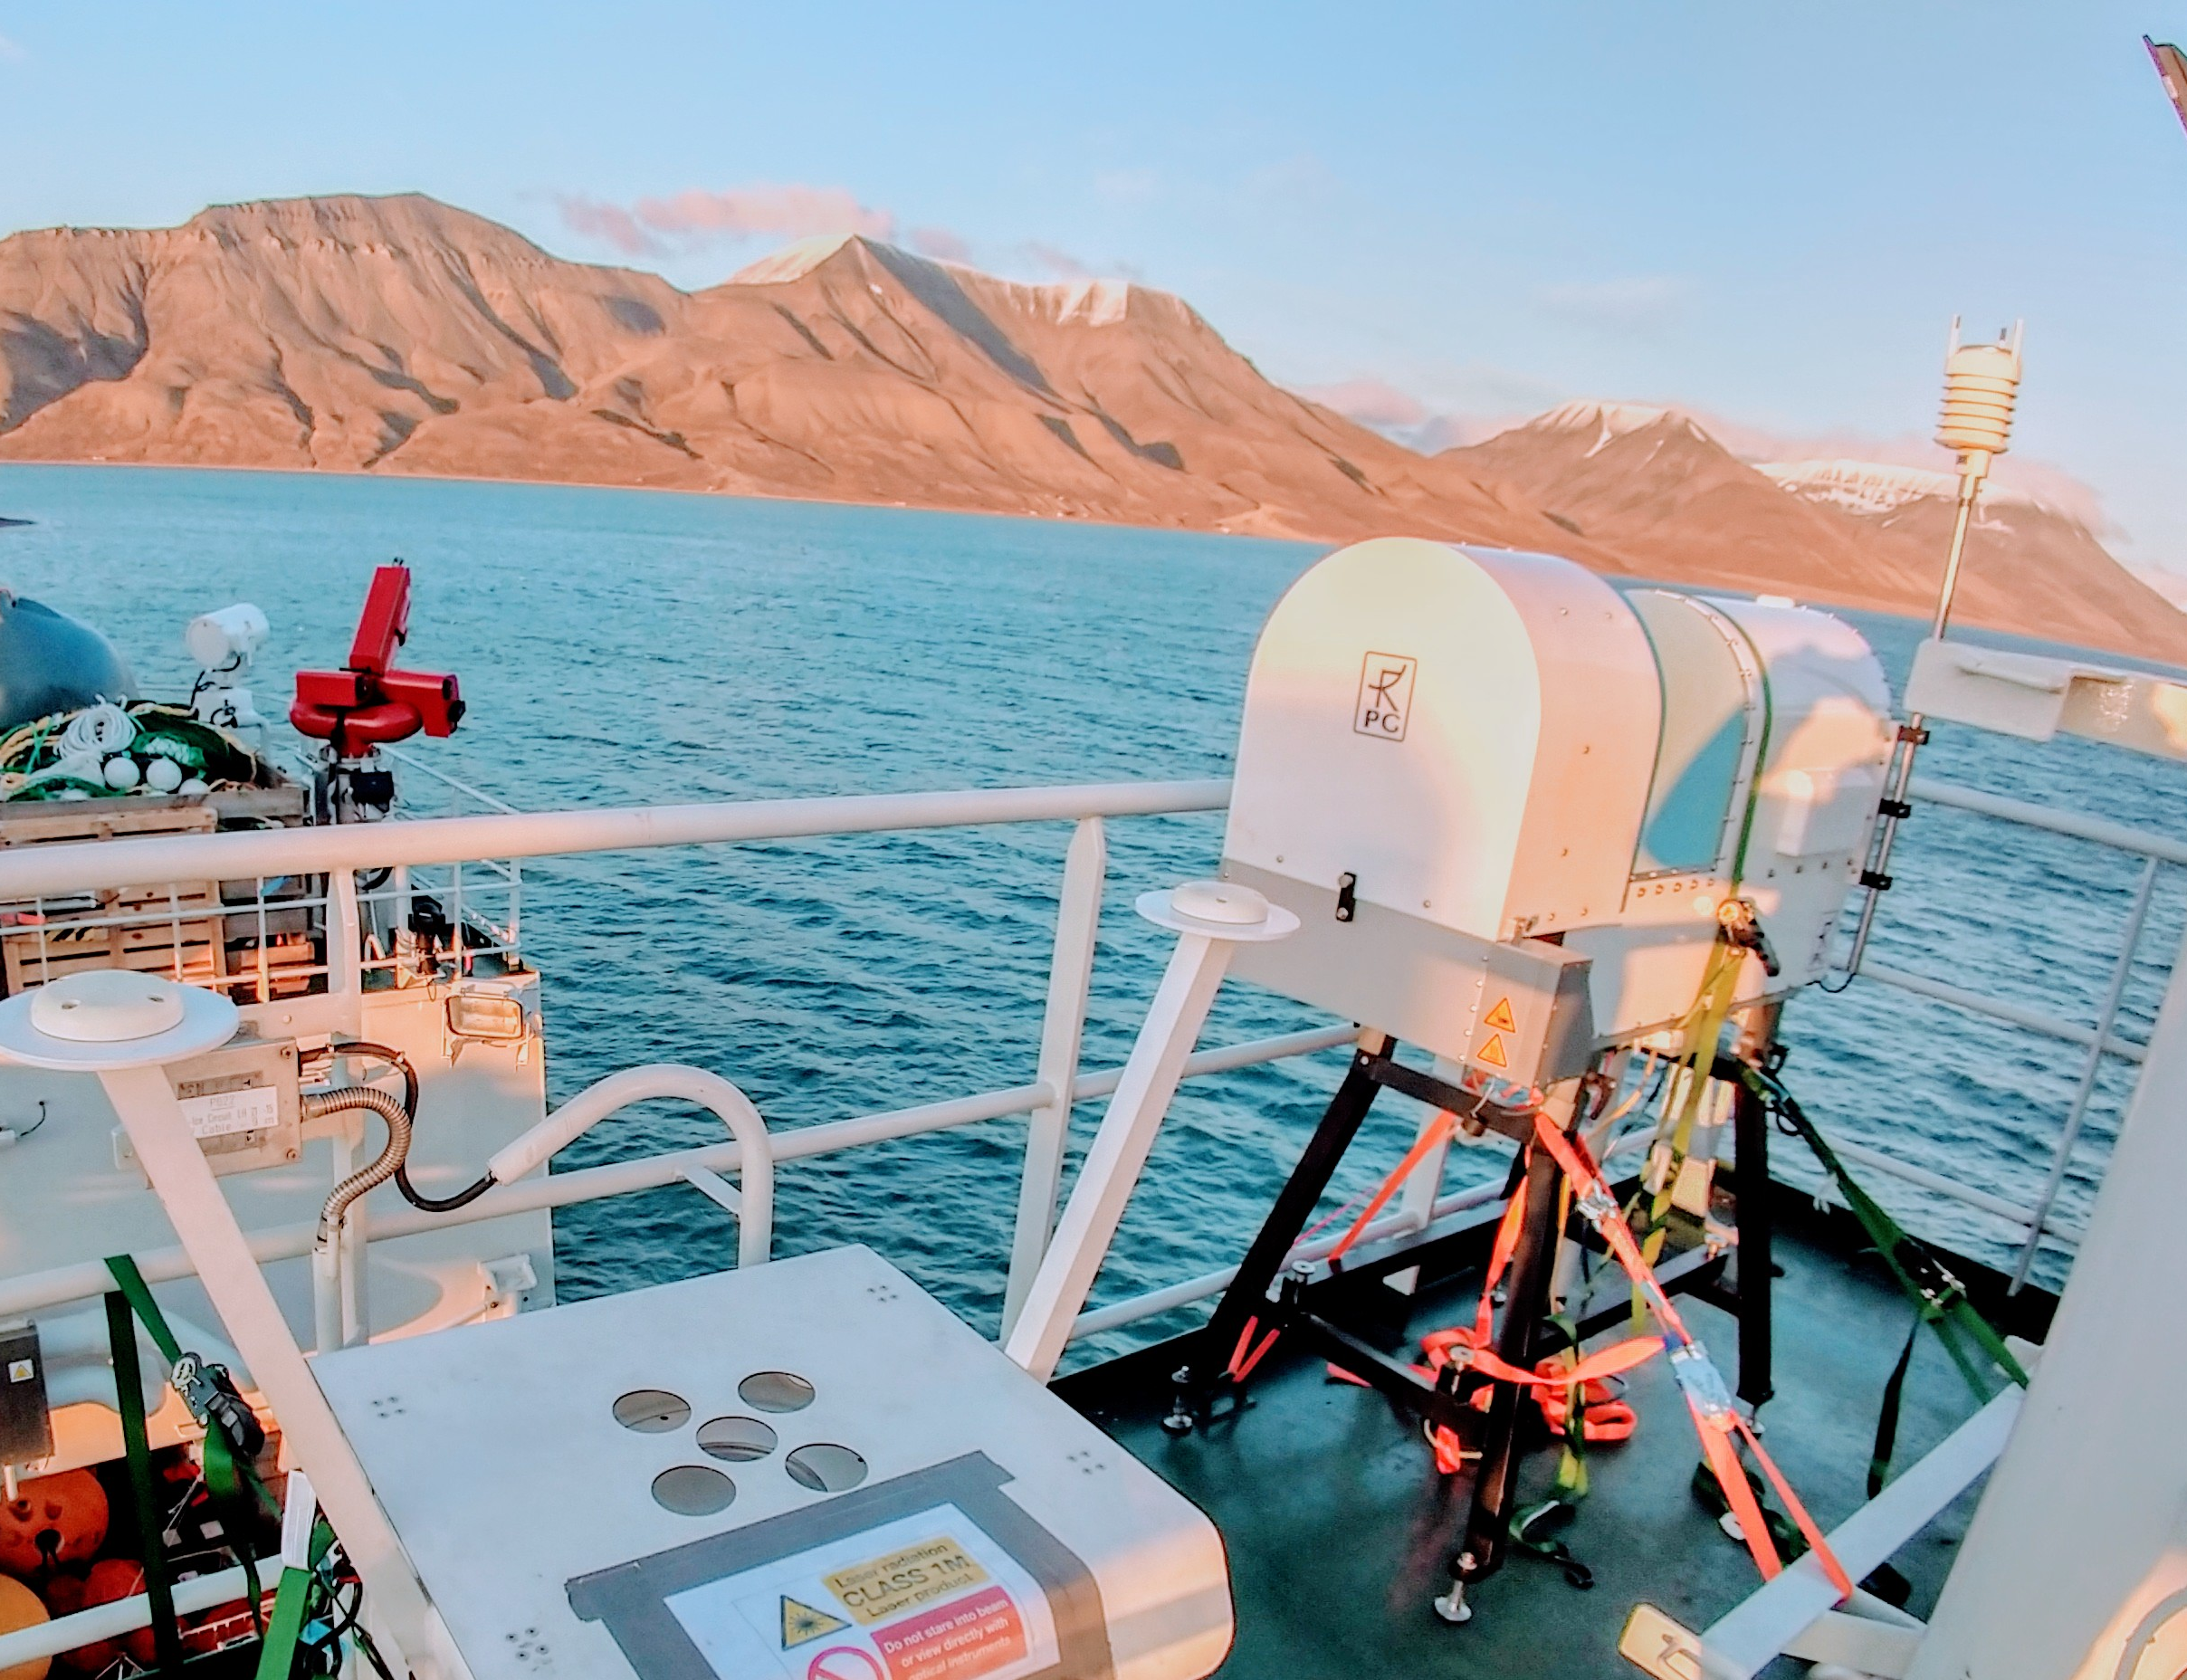
\includegraphics[width=.59\linewidth]{Nansen_Hatpro_V2.png}
	\end{center}
	{\small During the Nansen Legacy Cruise in September 2018, the HATPRO Radiometer measured on the \textit{Kronprins Haakon} Research vessel.}
	\end{minipage}
	&
  \begin{minipage}{0.55\linewidth}
    \begin{center}
    	   \includegraphics[width=.75\linewidth]{NansenL_200918_BL.png}
      \\
%      {\vspace{-2px} \sc \small
      Retrievals from 20th Sept. 2018.
%      }
    \end{center}
  \end{minipage}
\end{tabular}
Special care must be taken on analysis the data due to wave-forcing changes on elevation angle and effects on retrievals.		
}
%%%%%%%%%%%%%%%%%%%%%%%%%%%%%%%%%%%%%%%%%%%%%%%%%%%%%%%%%%%%%%%%%%%%%%%%%%%%%%
\headerbox{5.- Conclusions}{name=conclusion,column=3,below=apply}{
%%%%%%%%%%%%%%%%%%%%%%%%%%%%%%%%%%%%%%%%%%%%%%%%%%%%%%%%%%%%%%%%%%%%%%%%%%%%%%
{\small Advantages of Bayesian and Likelihood inversion:\\
* To customize an \textit{a-priori} dataset suited for specific climatologies [4],\\
* BAY and MLE use the same \textit{a-priori} to perform retrievals simultaneously,\\
* Synergistic observations from other instruments can be included to increase retrieval capabilities.\\
The retrievals performance are based on synthetic brightness temperatures, hence instrument calibration/systematic errors are not considered.\\
We found the MLE method better to retrieve temperature while BAY is better for humidity profiles. However Bayesian is found to be more sensitive to observation line-of-sight misalignments, where the RPG firmware shows to be less affected.}
}
%%%%%%%%%%%%%%%%%%%%%%%%%%%%%%%%%%%%%%%%%%%%%%%%%%%%%%%%%%%%%%%%%%%%%%%%%%%%%%
\headerbox{6.- References / Acknowledges}{name=references,column=3,above=bottom}{
%%%%%%%%%%%%%%%%%%%%%%%%%%%%%%%%%%%%%%%%%%%%%%%%%%%%%%%%%%%%%%%%%%%%%%%%%%%%%%
%\colouredcircle \hspace{2em}
\hspace{-2.4em}
\begin{minipage}{0.99\linewidth}
{\scriptsize
	\begin{enumerate}
		\item Inverse Methods for Atmospheric Sounding. Rodgers C.D. 2015. https://doi.org/10.1142/3171.
		\item \vspace{-0.4em} Bayesian Analysis in Inverse Problems, Fitzpatrick B.G. 1991. Inverse Problems 7, 675-702.
		\item \vspace{-0.4em} Instrument Operation \& Software guide, Issure 01/09, 2014. Radiometer Physics GmbH.
		\item \vspace{-0.4em} Wyoming Radiosonde Download Toolbox: http://www.github.com/pablosaa/WyoSonde
		\item \vspace{-0.4em} Bayes Retrieval Toolbox: http://www.github.com/pablosaa/TROPROS\_prof
	\end{enumerate}
}	
\vspace{-0.6em}
\end{minipage}\\
{\footnotesize
\textbf{Acknowledge} This work is performed as part of the Off-shore Boundary Layer Observatory (OBLO) and Bergen Off-shore Wind center (BOW). The authors thank to the University of Wyoming for making global radiosonde data available.}
	%\end{tabular}
	%\vspace{0.5em}
}


\end{poster}

\end{document}

%%%%%%%%%%%%%%%%%%%%%%%%%%%%%%%%%%%%%%%%%%%%%%%%%%%%%%%%%%%%%%%%%%%%%%%%%%%%%%%
%\headerbox{6. References}{name=ref,column=4,above=bottom,span=1}{%
%	%%%%%%%%%%%%%%%%%%%%%%%%%%%%%%%%%%%%%%%%%%%%%%%%%%%%%%%%%%%%%%%%%%%%%%%%%%%%%%
%	\begin{tabular}{@{}l||c@{}}
%		\hspace{-1.2em}
%		\begin{minipage}{0.35\linewidth}
%			%\vspace{-9em}
%			{Virtual Observations (VO) are needed to test Data Assimilation schemes. In that sense, synthetic observations alike SMAP/SMOS satellites have been generated. For that task, satellite features like orbit, antenna pattern, foot-print, incidence angle have been taking into account.}\\
%			%{\color{yellow} The statistics comprise of pixels within the Neckar catchment D4 after antenna pattern and real-orbit considerations. TOP PANEL: descending-orbit; BOTTOM PANEL: ascending-orbit.}
%			\vspace{-1.5em}
%			\begin{center}
%				%\includegraphics[width=.45\linewidth,height=115px]{img_lwc_10:30.png} &
%				\includegraphics[width=.5\linewidth]{AntennaPattern.png}
%			\end{center}
%			The above antenna pattern is a proxy for SMAP specifications, with a 3dB FWHM FOV of 2.4° and footprint of 36km. The pattern is applied to the high-resolution D4 simulations and SMAP Passive L2C\_TB\_PA synthetic data is generated.
%		\end{minipage}
%		%\vspace{-4em}
%		&
%		\begin{minipage}{0.6\linewidth}
%			\vspace{-0.1em}
%			\begin{center}
%				The synthetic observations are rendered according to the EASE-grid corresponding for the D4 catchment geo-locations i.e. 36km grid a like SMAP L2 data.\\
%				%     \hspace{-5em}
%				\includegraphics[scale=.5]{TBHcube_CLM_SAT.png}\\
%				{\color{red} SMAP virtual observations:} in the above figure the bottom-plane corresponds to TB high-res (206x234), while the top-plane the TB at EASE-grid D4 resolution (6x6). 
%				
%				%\includegraphics[width=.95\linewidth]{cmem_smosDA_BoxP2013.png}
%				%      \\
%				%      {\vspace{-2px} \sc \small
%				%      The Optical thicknesses retrieved from. 
%				%      }
%			\end{center}
%			%\vspace{8cm}
%		\end{minipage}
%	\end{tabular}\\
%	\begin{minipage}{0.98\linewidth}
%		\vspace{+0.2em}
%		\centering
%		\includegraphics[width=0.85\linewidth,height=7cm]{summer_TBclmSmap_ts.png}
%	\end{minipage}
%}
%%%%%%%%%%%%%%%%%%%%%%%%%%%%%%%%%%%%%%%%%%%%%%%%%%%%%%%%%%%%%%%%%%%%%%%%%%%%%%%
%\headerbox{7. Soil Moisture Bias in CLM}{name=clmbias,column=2,below=cmemout,span=2}{%
%	%%%%%%%%%%%%%%%%%%%%%%%%%%%%%%%%%%%%%%%%%%%%%%%%%%%%%%%%%%%%%%%%%%%%%%%%%%%%%%
%	\begin{tabular}{@{}c||c@{}}
%		\begin{minipage}{0.5\linewidth}
%			%\vspace{-9em}
%			{CLM shows large values for soil moisture, which leads to huge bias on TB. CDF matching method used to correct SM with real SMAP retrievals as reference (left plot). To understand the effects on TB by decreasing SM, various factors $\eta$ has been used to fit a curve (rigth plot)}\\
%			\vspace{-1.2em}
%			\begin{center}
%				\includegraphics[width=.48\linewidth]{cdfSM_clm_smap.png} \hspace{0.01cm}
%				\includegraphics[width=.49\linewidth]{deltaTB_fSM.png}
%			\end{center}
%			It has been found that CLM soil moisture values are in average 45\% ($\eta$=0.55) higher than SMAP retrievals for 1 year comparison. Then the factor $\eta$ is used to calibrate soil moisture to input the forward operator.
%		\end{minipage}
%		&
%		\begin{minipage}{0.44\linewidth}
%			{After calibration for Soil Moisture, the TB bias is partially reduced but not completely: The following plots are biases in a pixel-to-pixel comparison from VR and SMAP data after an average catchment bias is subtracted. The color of the EASE-grid pixel indicates residual bias and the value inside every circle is its respective ubRMSE.}\\
%			\vspace{-.2em}
%			\begin{center}
%				\includegraphics[width=.495\linewidth]{DIFF_TBH_VRD4_SMAP.png}\hspace{0.01cm}
%				\includegraphics[width=.495\linewidth]{DIFF_TBV_VRD4_SMAP.png}
%			\end{center}
%		\end{minipage}\\
%		\hline
%	\end{tabular}\\
%	
%	\begin{minipage}{0.95\linewidth}
%		\vspace{+.7em}
%		{\color{green} CONCLUSIONS:} 
%		It has been found that Bayesian inversion is able to more accurately reproduce the profiles vertical structure in contrast to the firmware retrieval methods. This is primary true for the case of humidity and temperature profiles.
%		%Moreover cases of synergy with a wind profiler are applied to the Bayesian scheme producing a consistent temperature, humidity and lower atmosphere wind shears simultaneously.
%		
%		The presented methodology for ground-based atmospheric profiling produces results resembling observations by radiosondes when a suitable a-priori dataset is used. Moreover the open source tools needed to produce the a-priori dataset for the Bayesian inversion is available on to be used by the scientific community.
%	\end{minipage}
%}
